\chapter{Task \#30: Axelrod model for dissemination of culture}

\section{Introduction}
The Axelrod model is an agent-based model used to study how social influence shapes cultural traits in individuals. In this context, the term ``culture'' refers to a set of traits, beliefs, or characteristics that an agent possesses and that may be shared or modified through interactions with neighboring agents \cite{axelrod_introduction}. The more similar these traits are, the more likely two neighboring agents will interact.

The objective of this model is to investigate how, and under what conditions, interactions between individual agents can create regions with a shared culture (consensus) as opposed to regions with different cultures (polarization) \cite{axelrod_algorithm}. Agent-based modeling provides a bottom-up approach in which global effects emerge from local interactions governed by a precise set of rules \cite{axelrod_introduction}.

The Axelrod model considers $N$ agents as nodes of a network (or lattice). Each agent $i$ has a vector of $F$ cultural features, $i = (i_1, i_2, \dots, i_F)$, where each feature $i_f$ can take one of $q$ integer values ($1, \dots, q$), initially assigned independently with equal probability $1/q$. The system evolves in discrete time steps as follows \cite{axelrod_algorithm}:

\begin{enumerate}
    \item A connected pair of agents $(i, j)$ is selected at random.
    \item The overlap $l_{ij}$, i.e., the number of shared features, is computed.
    \item If $0 < l_{ij} < F$, the link is \textbf{active}, and $i$ and $j$ interact with probability $l_{ij}/F$. In that case, a feature $g$ for which $i_g \neq j_g$ is selected randomly, and the corresponding value of $i$ is updated: $i_g = j_g$.
\end{enumerate}

The model has $q^F$ possible cultural configurations. Consensus is reached when a single configuration occupies the entire network; otherwise, the system is polarized. To quantify the system's state, we measure the size of the largest cultural domain, $S_{\max}$, often normalized by $N$. Here, $S_{\max}$ is defined as the size of the largest connected component of agents sharing the same culture.

This model is notable because, for a fixed $F$, there exists a critical value of $q$, denoted $q_c$, at which the system undergoes a phase transition from consensus to polarization, with $S_{\max}/N$ as the order parameter and $q$ as the control parameter \cite{axelrod_phase_transition}.

\section{Numerical simulations}
Given the goal of this model, the dynamics have been studied under different synthetic and real topologies (see Supplementary Material for this last one), with a fixed number of cultural features $F = 5$. In particular, regarding the synthetic networks ($N$ denotes the number of nodes):
\begin{itemize}
    \item \textbf{Erd\H{o}s-Rényi network:} $N = 1000$ and $p = 0.01$;
    \item \textbf{Barab\'asi-Albert network:} $N = 1000$ and $m = 5$;
    \item \textbf{Watts-Strogatz network:} $N = 1000$, $nei = 5$, and $p_{ws} = 0.03$ (where $nei$ is the number of neighbors for each node and $p_{ws}$ is the rewiring probability).
\end{itemize}
For 10 runs of $2 \times 10^7$ iterations each, we tracked the number of active links (referred to as "bonds" in the plots), $n_A$, and the size of the largest cultural domain, $S_{\max}$. On the left, we show the evolution of these quantities throughout the dynamics, while on the right, a phase transition plot is presented.

\begin{figure}[htbp]
    \centering
    \begin{minipage}{0.58\textwidth}
        \centering
        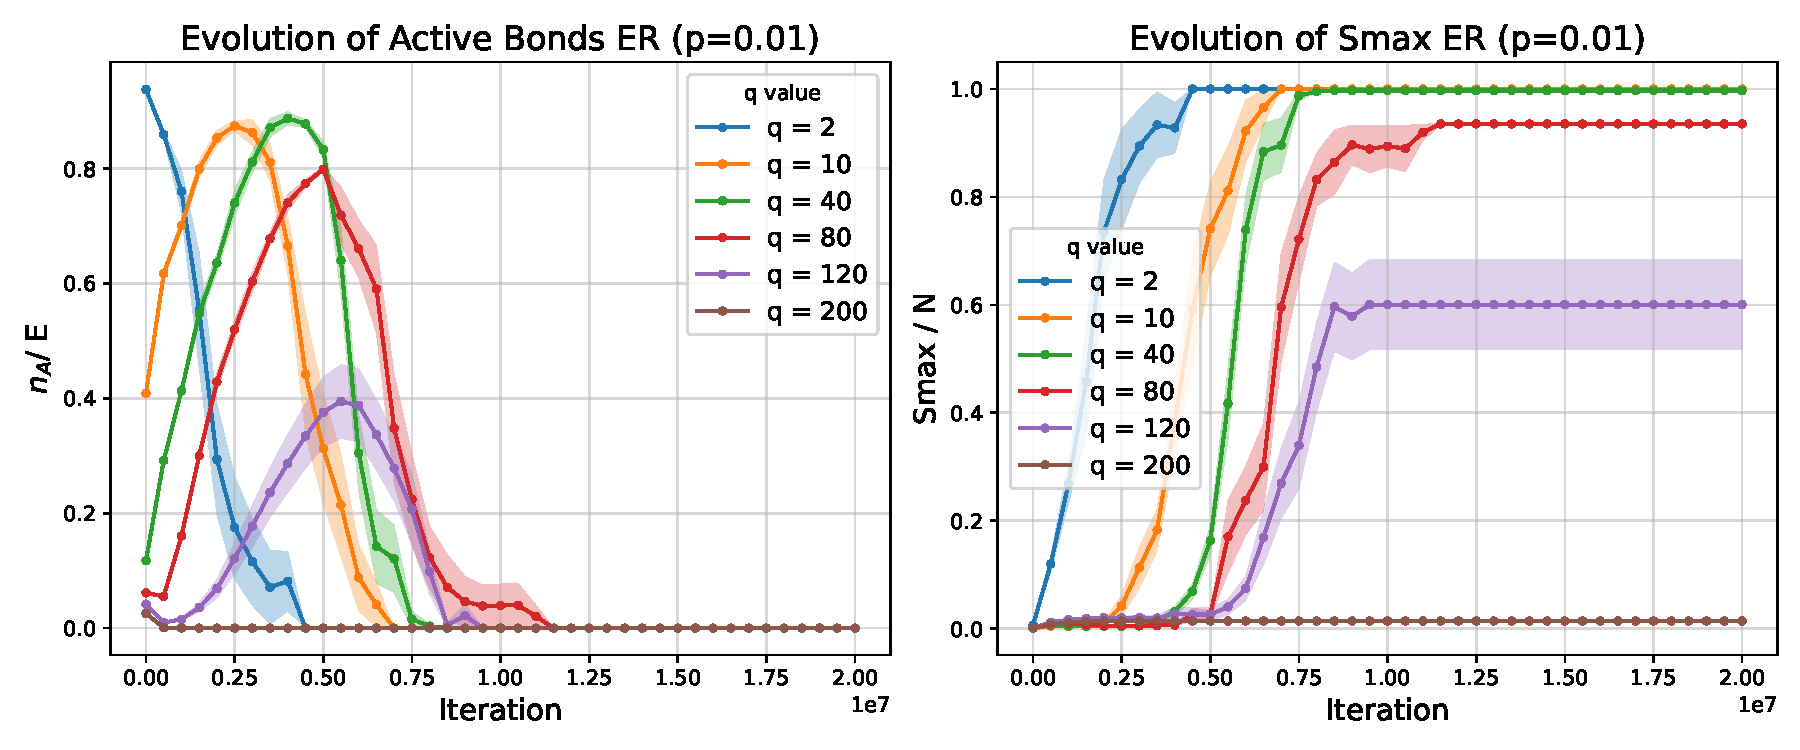
\includegraphics[width=1.\textwidth]{figures/task30_plots/evolution_plot_ER.pdf}
        %\caption{First plot}
    \end{minipage}
    \hfill
    \begin{minipage}{0.4\textwidth}
        \centering
        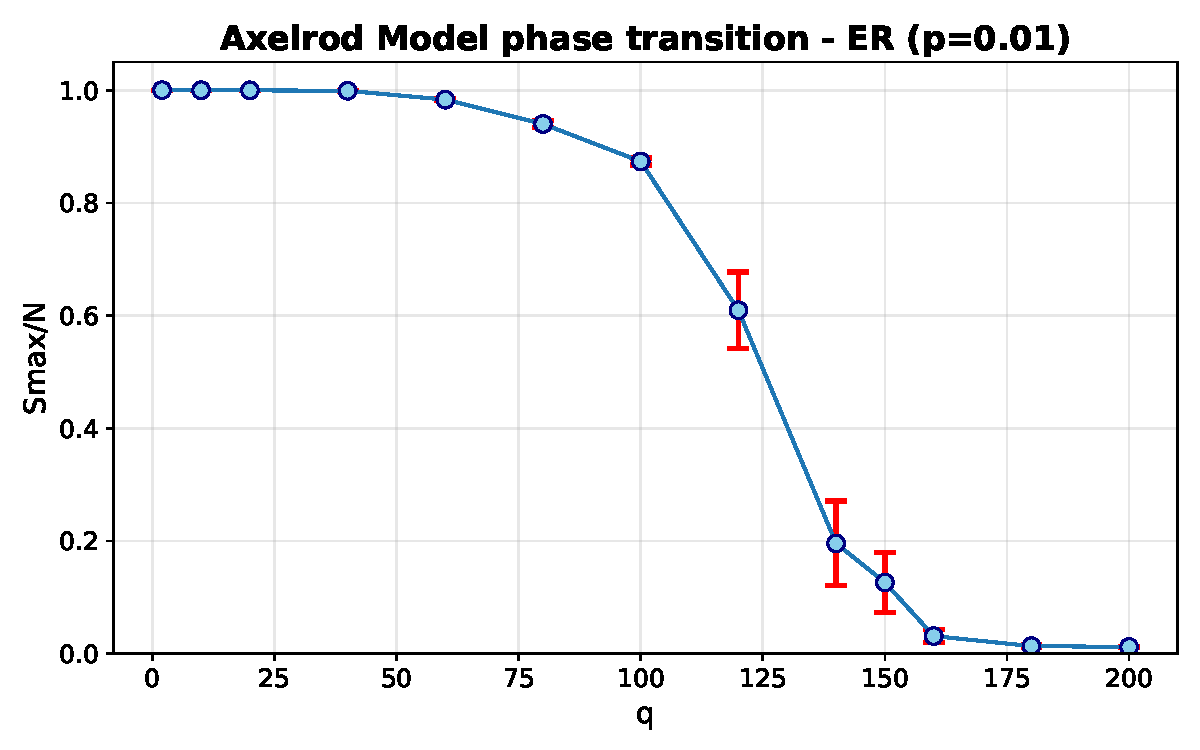
\includegraphics[width=0.9\textwidth]{figures/task30_plots/phase_transition_ER.pdf}
        %\caption{Second plot}
    \end{minipage}
\end{figure}

\begin{figure}[htbp]
    \centering
    \begin{minipage}{0.58\textwidth}
        \centering
        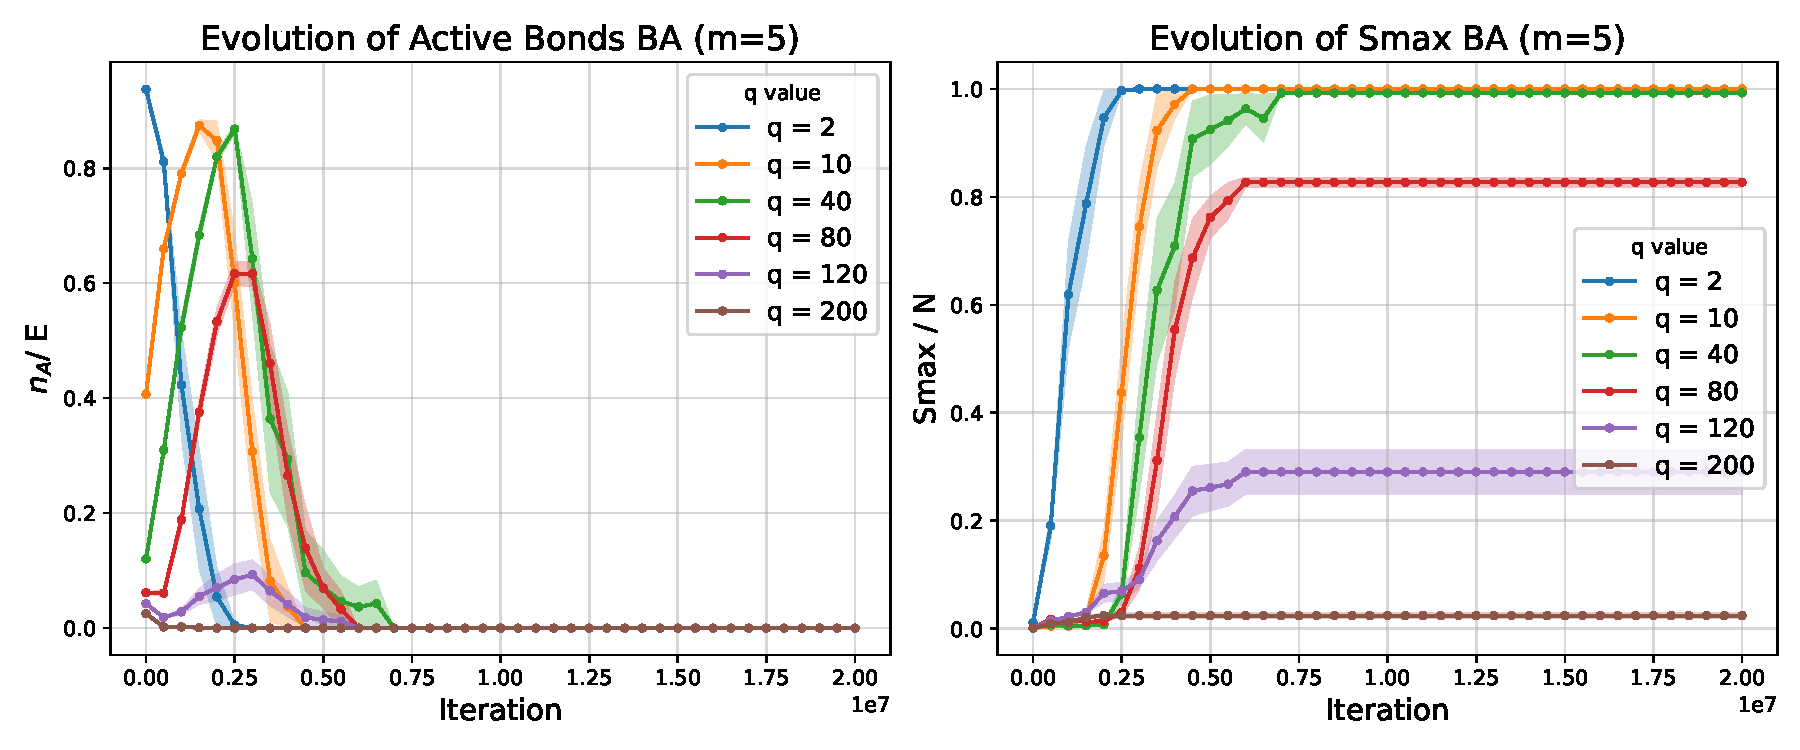
\includegraphics[width=1.\textwidth]{figures/task30_plots/evolution_plot_BA.pdf}
        \end{minipage}
    \hfill
    \begin{minipage}{0.4\textwidth}
        \centering
        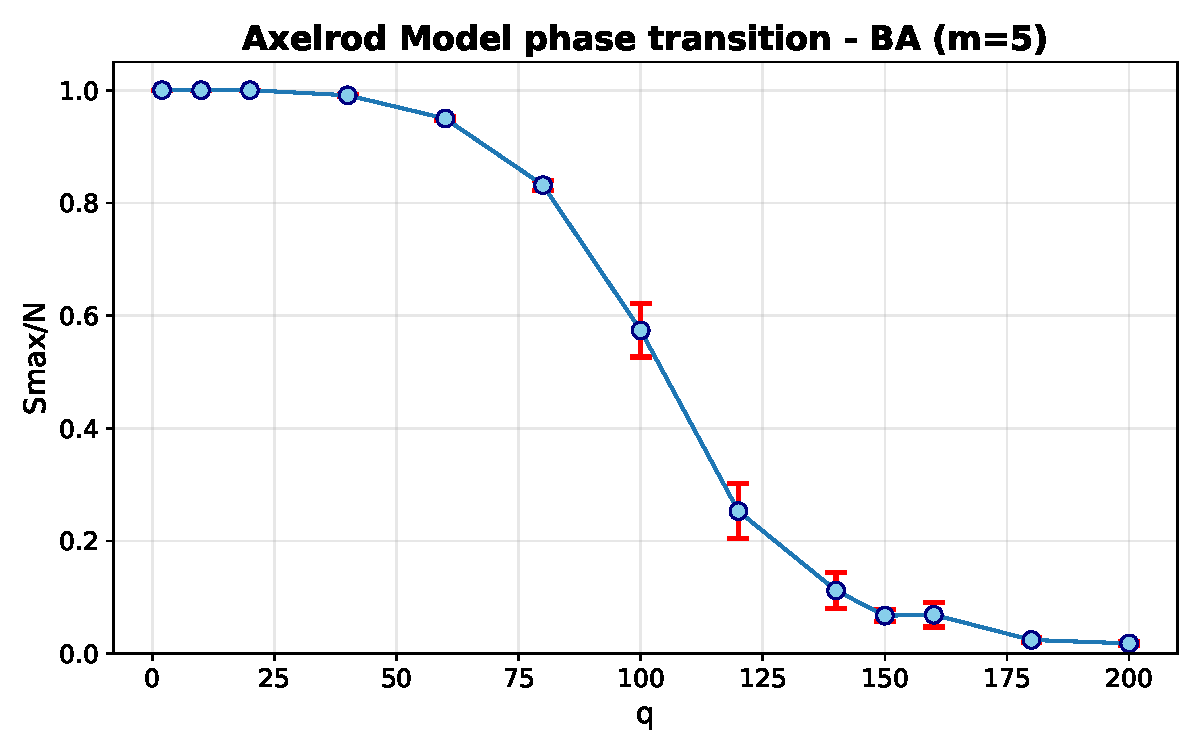
\includegraphics[width=0.9\textwidth]{figures/task30_plots/phase_transition_BA.pdf}
    \end{minipage}
\end{figure}

\begin{figure}[htbp]
    \centering
    \begin{minipage}{0.58\textwidth}
        \centering
        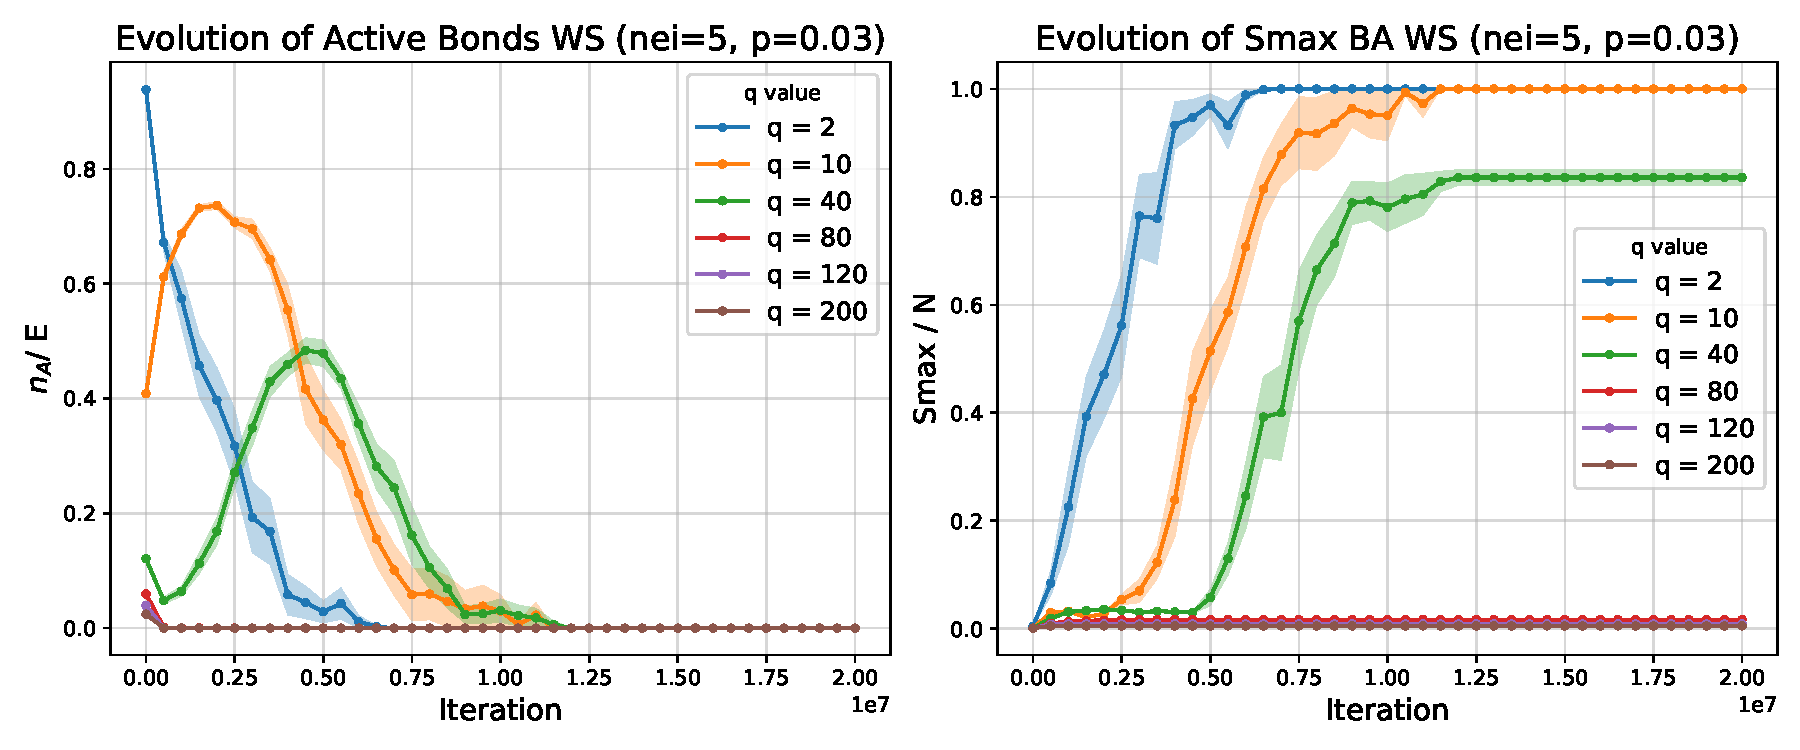
\includegraphics[width=1.\textwidth]{figures/task30_plots/evolution_plot_WS.pdf}
        %\caption{First plot}
    \end{minipage}
    \hfill
    \begin{minipage}{0.4\textwidth}
        \centering
        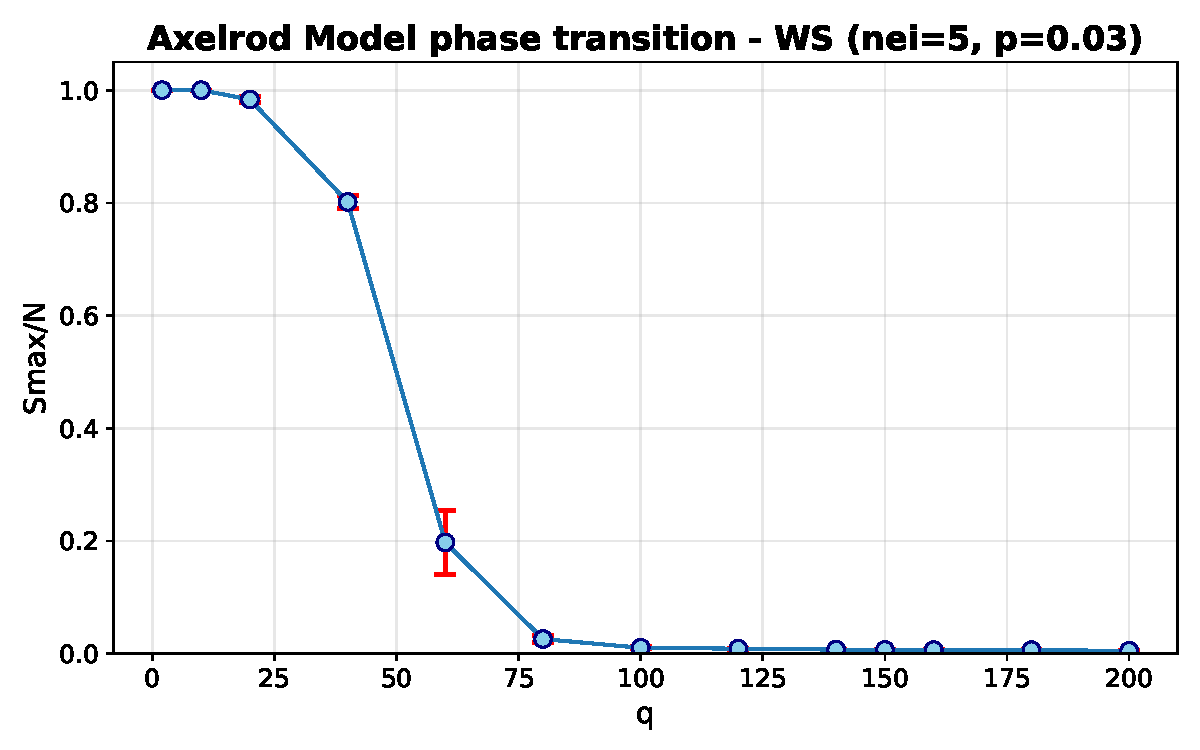
\includegraphics[width=0.9\textwidth]{figures/task30_plots/phase_transition_WS.pdf}
        %\caption{Second plot}
    \end{minipage}
\end{figure}
The simulation results show that network topology strongly affects the critical threshold for cultural polarization, with scale-free networks promoting consensus more effectively than random or small-world networks. Low $q$ values lead to rapid equilibration and consensus (active links decay quickly to zero), while high $q$ values ($q > q_c$) produce persistent cultural boundaries, with active links remaining non-zero for extended periods. A natural extension is to repeat the simulations on larger networks to reduce finite-size effects and to explore how varying model parameters influences the results.



\newpage